\documentclass{standalone}
\usepackage{tikz}
\usetikzlibrary{patterns, positioning}


\begin{document}
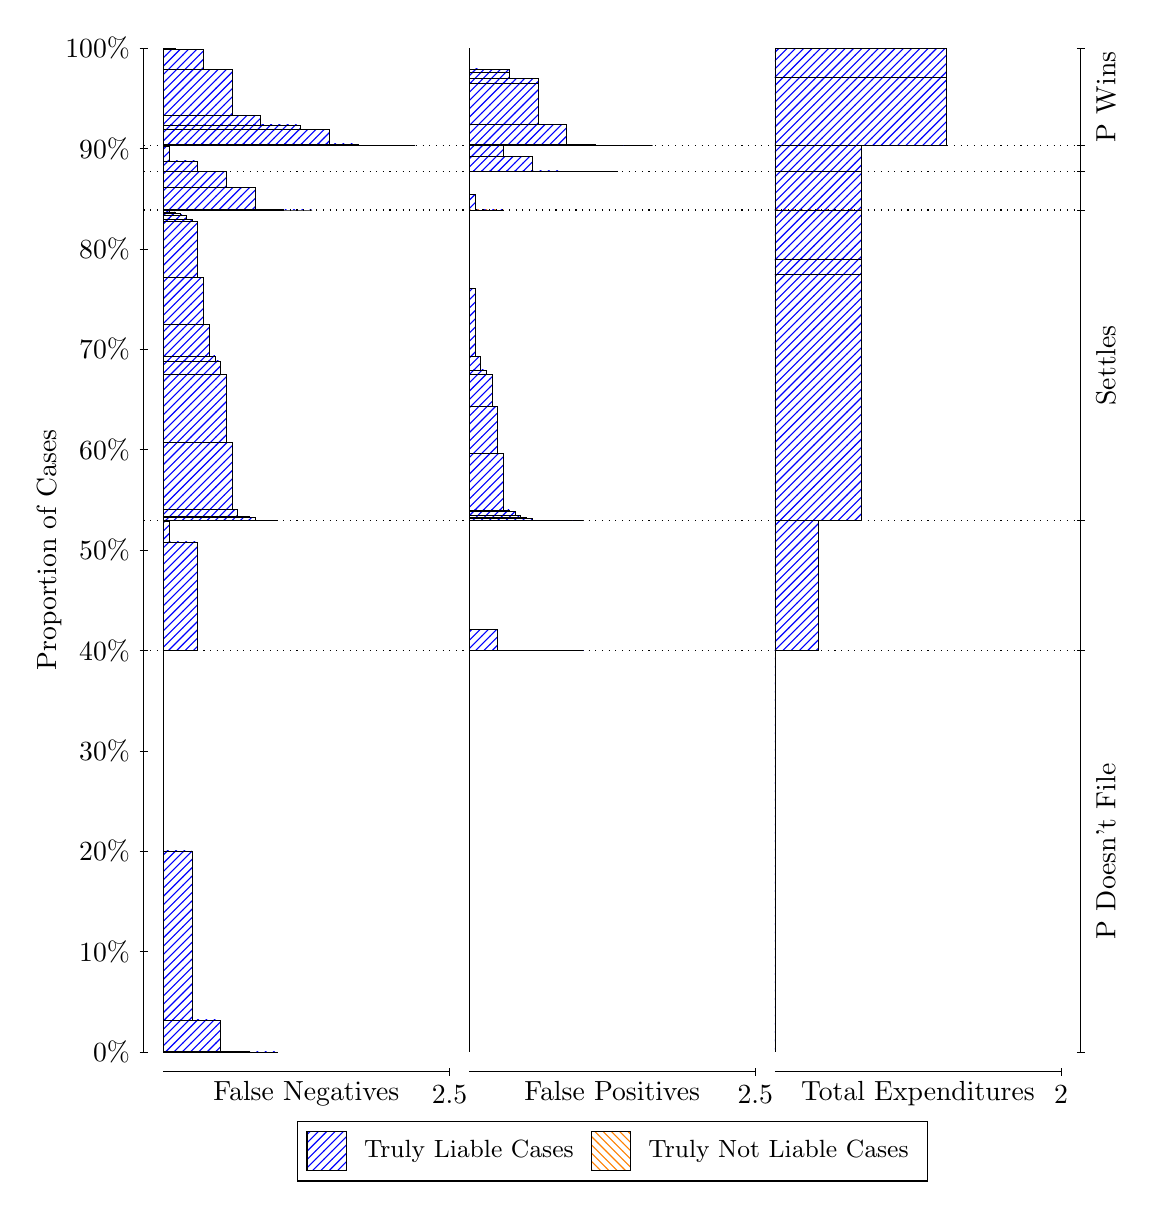
\begin{tikzpicture}
\draw[black, very thin] (1.5,1.75) -- (1.5,14.5);
\node[rotate=90, text=black, anchor=center] at (0.3, 8.125) {Proportion of Cases};
\draw[black, very thin] (1.45,1.75) -- (1.55,1.75);
\node[text=black, anchor=east] at (1.45, 1.75) {0\%};
\draw[black, very thin] (1.45,3.025) -- (1.55,3.025);
\node[text=black, anchor=east] at (1.45, 3.025) {10\%};
\draw[black, very thin] (1.45,4.3) -- (1.55,4.3);
\node[text=black, anchor=east] at (1.45, 4.3) {20\%};
\draw[black, very thin] (1.45,5.575) -- (1.55,5.575);
\node[text=black, anchor=east] at (1.45, 5.575) {30\%};
\draw[black, very thin] (1.45,6.85) -- (1.55,6.85);
\node[text=black, anchor=east] at (1.45, 6.85) {40\%};
\draw[black, very thin] (1.45,8.125) -- (1.55,8.125);
\node[text=black, anchor=east] at (1.45, 8.125) {50\%};
\draw[black, very thin] (1.45,9.4) -- (1.55,9.4);
\node[text=black, anchor=east] at (1.45, 9.4) {60\%};
\draw[black, very thin] (1.45,10.675) -- (1.55,10.675);
\node[text=black, anchor=east] at (1.45, 10.675) {70\%};
\draw[black, very thin] (1.45,11.95) -- (1.55,11.95);
\node[text=black, anchor=east] at (1.45, 11.95) {80\%};
\draw[black, very thin] (1.45,13.225) -- (1.55,13.225);
\node[text=black, anchor=east] at (1.45, 13.225) {90\%};
\draw[black, very thin] (1.45,14.5) -- (1.55,14.5);
\node[text=black, anchor=east] at (1.45, 14.5) {100\%};

\draw[black, very thin] (13.4,1.75) -- (13.4,14.5);
\draw[black, very thin] (13.35,1.75) -- (13.45,1.75);
\node[anchor=west] at (13.35, 1.75) {};
\draw[black, very thin] (13.35,6.8489) -- (13.45,6.8489);
\node[anchor=west] at (13.35, 6.8489) {};
\draw[black, very thin] (13.35,8.4976) -- (13.45,8.4976);
\node[anchor=west] at (13.35, 8.4976) {};
\draw[black, very thin] (13.35,12.443) -- (13.45,12.443);
\node[anchor=west] at (13.35, 12.443) {};
\draw[black, very thin] (13.35,12.935) -- (13.45,12.935);
\node[anchor=west] at (13.35, 12.935) {};
\draw[black, very thin] (13.35,13.259) -- (13.45,13.259);
\node[anchor=west] at (13.35, 13.259) {};
\draw[black, very thin] (13.35,14.5) -- (13.45,14.5);
\node[anchor=west] at (13.35, 14.5) {};

\draw[black, very thin, pattern color=blue, pattern=north east lines] (1.75,1.75) rectangle (3.2033,1.75);
\draw[black, very thin, pattern color=blue, pattern=north east lines] (1.75,1.75) rectangle (2.84,1.7534);
\draw[black, very thin, pattern color=blue, pattern=north east lines] (1.75,1.7534) rectangle (2.4767,2.158);
\draw[black, very thin, pattern color=blue, pattern=north east lines] (1.75,2.158) rectangle (2.1133,4.3029);
\draw[black, very thin, pattern color=orange, pattern=north west lines] (1.75,4.3029) rectangle (1.75,4.3029);
\draw[black, very thin, pattern color=blue, pattern=north east lines] (1.75,4.3029) rectangle (1.75,6.8489);
\draw[black, very thin, pattern color=blue, pattern=north east lines] (1.75,6.8489) rectangle (2.186,8.2282);
\draw[black, very thin, pattern color=blue, pattern=north east lines] (1.75,8.2282) rectangle (1.8227,8.4957);
\draw[black, very thin, pattern color=orange, pattern=north west lines] (1.75,8.4957) rectangle (1.75,8.4957);
\draw[black, very thin, pattern color=blue, pattern=north east lines] (1.75,8.4957) rectangle (1.75,8.4976);
\draw[black, very thin, pattern color=blue, pattern=north east lines] (1.75,8.4976) rectangle (3.2033,8.4976);
\draw[black, very thin, pattern color=blue, pattern=north east lines] (1.75,8.4976) rectangle (3.058,8.4978);
\draw[black, very thin, pattern color=blue, pattern=north east lines] (1.75,8.4978) rectangle (2.9127,8.5435);
\draw[black, very thin, pattern color=blue, pattern=north east lines] (1.75,8.5435) rectangle (2.84,8.5516);
\draw[black, very thin, pattern color=blue, pattern=north east lines] (1.75,8.5516) rectangle (2.7673,8.5524);
\draw[black, very thin, pattern color=blue, pattern=north east lines] (1.75,8.5524) rectangle (2.6947,8.6438);
\draw[black, very thin, pattern color=blue, pattern=north east lines] (1.75,8.6438) rectangle (2.622,9.4911);
\draw[black, very thin, pattern color=blue, pattern=north east lines] (1.75,9.4911) rectangle (2.5493,10.359);
\draw[black, very thin, pattern color=blue, pattern=north east lines] (1.75,10.359) rectangle (2.4767,10.527);
\draw[black, very thin, pattern color=blue, pattern=north east lines] (1.75,10.527) rectangle (2.404,10.589);
\draw[black, very thin, pattern color=blue, pattern=north east lines] (1.75,10.589) rectangle (2.3313,10.987);
\draw[black, very thin, pattern color=blue, pattern=north east lines] (1.75,10.987) rectangle (2.2587,11.588);
\draw[black, very thin, pattern color=blue, pattern=north east lines] (1.75,11.588) rectangle (2.186,12.305);
\draw[black, very thin, pattern color=blue, pattern=north east lines] (1.75,12.305) rectangle (2.1133,12.329);
\draw[black, very thin, pattern color=blue, pattern=north east lines] (1.75,12.329) rectangle (2.0407,12.38);
\draw[black, very thin, pattern color=blue, pattern=north east lines] (1.75,12.38) rectangle (1.968,12.397);
\draw[black, very thin, pattern color=blue, pattern=north east lines] (1.75,12.397) rectangle (1.8953,12.418);
\draw[black, very thin, pattern color=blue, pattern=north east lines] (1.75,12.418) rectangle (1.8227,12.443);
\draw[black, very thin, pattern color=orange, pattern=north west lines] (1.75,12.443) rectangle (1.75,12.443);
\draw[black, very thin, pattern color=blue, pattern=north east lines] (1.75,12.443) rectangle (1.75,12.443);
\draw[black, very thin, pattern color=blue, pattern=north east lines] (1.75,12.443) rectangle (3.6393,12.443);
\draw[black, very thin, pattern color=blue, pattern=north east lines] (1.75,12.443) rectangle (3.276,12.45);
\draw[black, very thin, pattern color=blue, pattern=north east lines] (1.75,12.45) rectangle (2.9127,12.733);
\draw[black, very thin, pattern color=blue, pattern=north east lines] (1.75,12.733) rectangle (2.5493,12.933);
\draw[black, very thin, pattern color=blue, pattern=north east lines] (1.75,12.933) rectangle (2.186,12.935);
\draw[black, very thin, pattern color=orange, pattern=north west lines] (1.75,12.935) rectangle (1.75,12.935);
\draw[black, very thin, pattern color=blue, pattern=north east lines] (1.75,12.935) rectangle (2.186,13.068);
\draw[black, very thin, pattern color=blue, pattern=north east lines] (1.75,13.068) rectangle (1.8227,13.253);
\draw[black, very thin, pattern color=orange, pattern=north west lines] (1.75,13.253) rectangle (1.75,13.253);
\draw[black, very thin, pattern color=blue, pattern=north east lines] (1.75,13.253) rectangle (1.75,13.259);
\draw[black, very thin, pattern color=blue, pattern=north east lines] (1.75,13.259) rectangle (4.9473,13.259);
\draw[black, very thin, pattern color=blue, pattern=north east lines] (1.75,13.259) rectangle (4.584,13.259);
\draw[black, very thin, pattern color=blue, pattern=north east lines] (1.75,13.259) rectangle (4.2207,13.284);
\draw[black, very thin, pattern color=blue, pattern=north east lines] (1.75,13.284) rectangle (3.8573,13.467);
\draw[black, very thin, pattern color=blue, pattern=north east lines] (1.75,13.467) rectangle (3.712,13.467);
\draw[black, very thin, pattern color=blue, pattern=north east lines] (1.75,13.467) rectangle (3.494,13.525);
\draw[black, very thin, pattern color=blue, pattern=north east lines] (1.75,13.525) rectangle (3.3487,13.525);
\draw[black, very thin, pattern color=blue, pattern=north east lines] (1.75,13.525) rectangle (3.1307,13.525);
\draw[black, very thin, pattern color=blue, pattern=north east lines] (1.75,13.525) rectangle (2.9853,13.642);
\draw[black, very thin, pattern color=blue, pattern=north east lines] (1.75,13.642) rectangle (2.7673,13.642);
\draw[black, very thin, pattern color=blue, pattern=north east lines] (1.75,13.642) rectangle (2.622,14.23);
\draw[black, very thin, pattern color=blue, pattern=north east lines] (1.75,14.23) rectangle (2.2587,14.486);
\draw[black, very thin, pattern color=blue, pattern=north east lines] (1.75,14.486) rectangle (1.8953,14.5);
\draw[black, very thin, pattern color=orange, pattern=north west lines] (1.75,14.5) rectangle (1.75,14.5);
\draw[black, very thin, pattern color=blue, pattern=north east lines] (1.75,14.5) rectangle (1.75,14.5);
\draw[black, very thin, pattern color=orange, pattern=north west lines] (5.6333,1.75) rectangle (5.6333,1.75);
\draw[black, very thin, pattern color=blue, pattern=north east lines] (5.6333,1.75) rectangle (5.6333,6.8489);
\draw[black, very thin, pattern color=orange, pattern=north west lines] (5.6333,6.8489) rectangle (7.0867,6.8489);
\draw[black, very thin, pattern color=blue, pattern=north east lines] (5.6333,6.8489) rectangle (7.0867,6.8489);
\draw[black, very thin, pattern color=blue, pattern=north east lines] (5.6333,6.8489) rectangle (6.7233,6.8489);
\draw[black, very thin, pattern color=blue, pattern=north east lines] (5.6333,6.8489) rectangle (6.36,6.8508);
\draw[black, very thin, pattern color=blue, pattern=north east lines] (5.6333,6.8508) rectangle (5.9967,7.1182);
\draw[black, very thin, pattern color=blue, pattern=north east lines] (5.6333,7.1182) rectangle (5.6333,8.4976);
\draw[black, very thin, pattern color=orange, pattern=north west lines] (5.6333,8.4976) rectangle (7.0867,8.4976);
\draw[black, very thin, pattern color=blue, pattern=north east lines] (5.6333,8.4976) rectangle (7.0867,8.4976);
\draw[black, very thin, pattern color=orange, pattern=north west lines] (5.6333,8.4976) rectangle (6.9413,8.4976);
\draw[black, very thin, pattern color=blue, pattern=north east lines] (5.6333,8.4976) rectangle (6.9413,8.4976);
\draw[black, very thin, pattern color=orange, pattern=north west lines] (5.6333,8.4976) rectangle (6.796,8.4976);
\draw[black, very thin, pattern color=blue, pattern=north east lines] (5.6333,8.4976) rectangle (6.796,8.4976);
\draw[black, very thin, pattern color=blue, pattern=north east lines] (5.6333,8.4976) rectangle (6.7233,8.4976);
\draw[black, very thin, pattern color=orange, pattern=north west lines] (5.6333,8.4976) rectangle (6.6507,8.4976);
\draw[black, very thin, pattern color=blue, pattern=north east lines] (5.6333,8.4976) rectangle (6.6507,8.4976);
\draw[black, very thin, pattern color=blue, pattern=north east lines] (5.6333,8.4976) rectangle (6.578,8.4977);
\draw[black, very thin, pattern color=orange, pattern=north west lines] (5.6333,8.4977) rectangle (6.5053,8.4977);
\draw[black, very thin, pattern color=blue, pattern=north east lines] (5.6333,8.4977) rectangle (6.5053,8.4978);
\draw[black, very thin, pattern color=blue, pattern=north east lines] (5.6333,8.4978) rectangle (6.4327,8.522);
\draw[black, very thin, pattern color=blue, pattern=north east lines] (5.6333,8.522) rectangle (6.36,8.5434);
\draw[black, very thin, pattern color=blue, pattern=north east lines] (5.6333,8.5434) rectangle (6.2873,8.5608);
\draw[black, very thin, pattern color=blue, pattern=north east lines] (5.6333,8.5608) rectangle (6.2147,8.6112);
\draw[black, very thin, pattern color=blue, pattern=north east lines] (5.6333,8.6112) rectangle (6.142,8.6352);
\draw[black, very thin, pattern color=blue, pattern=north east lines] (5.6333,8.6352) rectangle (6.0693,9.3522);
\draw[black, very thin, pattern color=blue, pattern=north east lines] (5.6333,9.3522) rectangle (5.9967,9.9535);
\draw[black, very thin, pattern color=blue, pattern=north east lines] (5.6333,9.9535) rectangle (5.924,10.351);
\draw[black, very thin, pattern color=blue, pattern=north east lines] (5.6333,10.351) rectangle (5.8513,10.413);
\draw[black, very thin, pattern color=blue, pattern=north east lines] (5.6333,10.413) rectangle (5.7787,10.581);
\draw[black, very thin, pattern color=blue, pattern=north east lines] (5.6333,10.581) rectangle (5.706,11.449);
\draw[black, very thin, pattern color=blue, pattern=north east lines] (5.6333,11.449) rectangle (5.6333,12.443);
\draw[black, very thin, pattern color=orange, pattern=north west lines] (5.6333,12.443) rectangle (6.0693,12.443);
\draw[black, very thin, pattern color=blue, pattern=north east lines] (5.6333,12.443) rectangle (6.0693,12.445);
\draw[black, very thin, pattern color=blue, pattern=north east lines] (5.6333,12.445) rectangle (5.706,12.646);
\draw[black, very thin, pattern color=blue, pattern=north east lines] (5.6333,12.646) rectangle (5.6333,12.935);
\draw[black, very thin, pattern color=orange, pattern=north west lines] (5.6333,12.935) rectangle (7.5227,12.935);
\draw[black, very thin, pattern color=blue, pattern=north east lines] (5.6333,12.935) rectangle (7.5227,12.935);
\draw[black, very thin, pattern color=blue, pattern=north east lines] (5.6333,12.935) rectangle (7.1593,12.935);
\draw[black, very thin, pattern color=blue, pattern=north east lines] (5.6333,12.935) rectangle (6.796,12.941);
\draw[black, very thin, pattern color=blue, pattern=north east lines] (5.6333,12.941) rectangle (6.4327,13.126);
\draw[black, very thin, pattern color=blue, pattern=north east lines] (5.6333,13.126) rectangle (6.0693,13.259);
\draw[black, very thin, pattern color=orange, pattern=north west lines] (5.6333,13.259) rectangle (7.9587,13.259);
\draw[black, very thin, pattern color=blue, pattern=north east lines] (5.6333,13.259) rectangle (7.9587,13.259);
\draw[black, very thin, pattern color=orange, pattern=north west lines] (5.6333,13.259) rectangle (7.5953,13.259);
\draw[black, very thin, pattern color=blue, pattern=north east lines] (5.6333,13.259) rectangle (7.5953,13.259);
\draw[black, very thin, pattern color=orange, pattern=north west lines] (5.6333,13.259) rectangle (7.232,13.259);
\draw[black, very thin, pattern color=blue, pattern=north east lines] (5.6333,13.259) rectangle (7.232,13.273);
\draw[black, very thin, pattern color=blue, pattern=north east lines] (5.6333,13.273) rectangle (6.8687,13.528);
\draw[black, very thin, pattern color=orange, pattern=north west lines] (5.6333,13.528) rectangle (6.8687,13.528);
\draw[black, very thin, pattern color=blue, pattern=north east lines] (5.6333,13.528) rectangle (6.8687,13.528);
\draw[black, very thin, pattern color=blue, pattern=north east lines] (5.6333,13.528) rectangle (6.5053,14.056);
\draw[black, very thin, pattern color=blue, pattern=north east lines] (5.6333,14.056) rectangle (6.5053,14.116);
\draw[black, very thin, pattern color=orange, pattern=north west lines] (5.6333,14.116) rectangle (6.36,14.116);
\draw[black, very thin, pattern color=blue, pattern=north east lines] (5.6333,14.116) rectangle (6.36,14.116);
\draw[black, very thin, pattern color=blue, pattern=north east lines] (5.6333,14.116) rectangle (6.142,14.191);
\draw[black, very thin, pattern color=blue, pattern=north east lines] (5.6333,14.191) rectangle (6.142,14.233);
\draw[black, very thin, pattern color=orange, pattern=north west lines] (5.6333,14.233) rectangle (5.9967,14.233);
\draw[black, very thin, pattern color=blue, pattern=north east lines] (5.6333,14.233) rectangle (5.9967,14.233);
\draw[black, very thin, pattern color=blue, pattern=north east lines] (5.6333,14.233) rectangle (5.7787,14.233);
\draw[black, very thin, pattern color=blue, pattern=north east lines] (5.6333,14.233) rectangle (5.7787,14.234);
\draw[black, very thin, pattern color=orange, pattern=north west lines] (5.6333,14.234) rectangle (5.6333,14.234);
\draw[black, very thin, pattern color=blue, pattern=north east lines] (5.6333,14.234) rectangle (5.6333,14.5);
\draw[black, very thin, pattern color=orange, pattern=north west lines] (9.5167,1.75) rectangle (9.5167,1.75);
\draw[black, very thin, pattern color=blue, pattern=north east lines] (9.5167,1.75) rectangle (9.5167,6.8489);
\draw[black, very thin, pattern color=orange, pattern=north west lines] (9.5167,6.8489) rectangle (10.062,6.8489);
\draw[black, very thin, pattern color=blue, pattern=north east lines] (9.5167,6.8489) rectangle (10.062,8.4976);
\draw[black, very thin, pattern color=orange, pattern=north west lines] (9.5167,8.4976) rectangle (10.607,8.4976);
\draw[black, very thin, pattern color=blue, pattern=north east lines] (9.5167,8.4976) rectangle (10.607,11.623);
\draw[black, very thin, pattern color=orange, pattern=north west lines] (9.5167,11.623) rectangle (10.607,11.623);
\draw[black, very thin, pattern color=blue, pattern=north east lines] (9.5167,11.623) rectangle (10.607,11.823);
\draw[black, very thin, pattern color=orange, pattern=north west lines] (9.5167,11.823) rectangle (10.607,11.823);
\draw[black, very thin, pattern color=blue, pattern=north east lines] (9.5167,11.823) rectangle (10.607,12.443);
\draw[black, very thin, pattern color=orange, pattern=north west lines] (9.5167,12.443) rectangle (10.607,12.443);
\draw[black, very thin, pattern color=blue, pattern=north east lines] (9.5167,12.443) rectangle (10.607,12.935);
\draw[black, very thin, pattern color=orange, pattern=north west lines] (9.5167,12.935) rectangle (10.607,12.935);
\draw[black, very thin, pattern color=blue, pattern=north east lines] (9.5167,12.935) rectangle (10.607,13.259);
\draw[black, very thin, pattern color=orange, pattern=north west lines] (9.5167,13.259) rectangle (11.697,13.259);
\draw[black, very thin, pattern color=blue, pattern=north east lines] (9.5167,13.259) rectangle (11.697,14.13);
\draw[black, very thin, pattern color=orange, pattern=north west lines] (9.5167,14.13) rectangle (11.697,14.13);
\draw[black, very thin, pattern color=blue, pattern=north east lines] (9.5167,14.13) rectangle (11.697,14.5);
\draw[black, dotted] (1.5,6.8489) -- (13.4,6.8489);
\draw[black, dotted] (1.5,8.4976) -- (13.4,8.4976);
\draw[black, dotted] (1.5,12.443) -- (13.4,12.443);
\draw[black, dotted] (1.5,12.935) -- (13.4,12.935);
\draw[black, dotted] (1.5,13.259) -- (13.4,13.259);
\draw[black, very thin] (1.75,1.5) -- (5.3833,1.5);
\node[text=black, anchor=north] at (3.5667, 1.5) {False Negatives};
\draw[black, very thin] (5.3833,1.45) -- (5.3833,1.55);
\node[text=black, anchor=north] at (5.3833, 1.45) {2.5};

\draw[black, very thin] (5.6333,1.5) -- (9.2667,1.5);
\node[text=black, anchor=north] at (7.45, 1.5) {False Positives};
\draw[black, very thin] (9.2667,1.45) -- (9.2667,1.55);
\node[text=black, anchor=north] at (9.2667, 1.45) {2.5};

\draw[black, very thin] (9.5167,1.5) -- (13.15,1.5);
\node[text=black, anchor=north] at (11.333, 1.5) {Total Expenditures};
\draw[black, very thin] (13.15,1.45) -- (13.15,1.55);
\node[text=black, anchor=north] at (13.15, 1.45) {2};

\node[text=black, centered, rotate=90] at (13.72, 4.2994) {P Doesn't File};

\node[text=black, centered, rotate=90] at (13.72, 10.47) {Settles};


\node[text=black, centered, rotate=90] at (13.72, 13.879) {P Wins};

\draw (7.449999999999999,1.5) node[draw=none] (baseCoordinate) {};
\begin{scope}[align=center]
        \matrix[scale=0.5, draw=black, below=0.5cm of baseCoordinate, nodes={draw}, column sep=0.1cm]{
            \node[rectangle, draw, minimum width=0.5cm, minimum height=0.5cm, pattern color=blue, pattern=north east lines] {}; &
            \node[draw=none, font=\small, text=black] (B) {Truly Liable Cases}; &
            \node[rectangle, draw, minimum width=0.5cm, minimum height=0.5cm, pattern color=orange, pattern=north west lines] {}; &
            \node[draw=none, font=\small, text=black] (B) {Truly Not Liable Cases}; \\
            };
\end{scope}

\end{tikzpicture}
\end{document}